\paragraph{QuizziPedia::Back-End::App::Models::QuestionModel}
\label{QuizziPedia::Back-End::App::Models::QuestionModel}
\begin{figure}
	\centering
	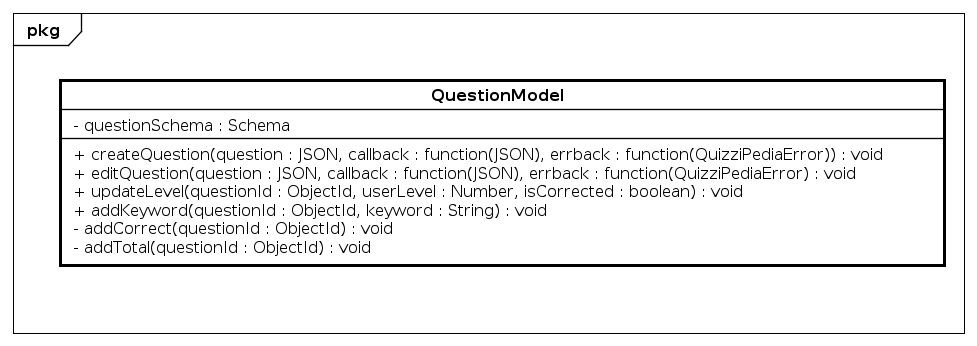
\includegraphics[scale=0.45]{UML/Package/QuizziPedia_Back-End_App_Models_questionModel.png}
	\caption{QuizziPedia::Back-End::App::Models::QuestionModel}
\end{figure}
\begin{itemize}
\item \textbf{Descrizione}: Questa classe rappresenta le domande;	
\item \textbf{Utilizzo}: Viene utilizzata per rappresentare le domande. Si interfaccia alla libreria Mongoose per la creazione dello schema e dei relativi metodi statici o di istanza;
\item \textbf{Relazione con altra classi}:
	\begin{itemize}
	\item IN UserModel;
	\item IN SummaryModel;
	\item OUT TopicModel;
	\item OUT QuizModel.
	\end{itemize}
\item \textbf{Attributi}:
	\begin{itemize}
	\item \texttt{questionSchema: Schema} \\
	Questo campo dati rappresenta lo schema Mongoose per le domande e prevede i 					seguenti attributi:
		\begin{itemize}
		\item \texttt{author} di tipo \texttt{ObjectId}, rappresenta il riferimento 					all'identificativo nel database dell'utente che ha creato la domanda;
		\item \texttt{type} di tipo \texttt{String}, rappresenta la tipologia di domanda;
		\item \texttt{questionText} di tipo \texttt{String}, rappresenta il testo della 				domanda; 
		\item \texttt{image} di tipo \texttt{String}, rappresenta l'URL dell'immagine 				associata al testo della domanda;
		\item \texttt{options1} di tipo \texttt{Array}, contiene oggetti di tipo String e 			rappresenta informazioni diverse in base alla tipologia della	 domanda;
		\item \texttt{options2} di tipo \texttt{Array}, contiene oggetti di tipo String e 			rappresenta informazioni diverse in base alla tipologia della	 domanda;
		\item \texttt{level} di tipo \texttt{Number}, rappresenta la difficoltà della 				domanda;
		\item \texttt{totalAnswers} di tipo \texttt{Number}, rappresenta le risposte 					totali che tutti gli utenti hanno dato alla domanda;
		\item \texttt{correctAnswers} di tipo \texttt{Number}, rappresenta quante risposte 		corrette hanno dato gli utenti che hanno risposto alla domanda.
		\end{itemize}
	\end{itemize}
\item \textbf{Metodi}:
	\begin{itemize}
	\item \texttt{+ createQuestion(content: JSON, callback: function(JSON))} \\
	;   
	\item \texttt{+ editQuestion(content: JSON, callback: function(JSON))} \\
	.
	\end{itemize}
\end{itemize}